\documentclass[12pt]{article}
\oddsidemargin -0.5in
\evensidemargin -0.5in
\textwidth 7.2in
\topmargin -0.5in
\textheight 8in
\flushbottom

\usepackage[authoryear,round]{natbib} %a package for formatting citations
\usepackage{amsmath} %a package for good looking equations and symbols
\usepackage{algorithm2e} %a package for typesetting algorithms
% \usepackage{caption} %a package for more complex captions for figures/tables/images
\usepackage{subcaption} %extension of the caption package
\usepackage{url} %embedded, clickable links
\usepackage{fullpage} %including this package changes the default margins to use more of the page
\usepackage{graphicx} %package for inline images
\usepackage[usenames]{xcolor} %for adding color text
\usepackage{enumitem} %for nested numbered lists (like in the questions section)
% \usepackage{hyperref}
% \usepackage{amsfonts}

\newcommand{\nextproblem}{
	\vfill
	\pagebreak
}


\begin{document}


	\begin{center}
			\textbf{CS 4641 Machine Learning} \vspace*{2mm}
			\textbf{\\ Bojun Yang | Section B} \vspace*{2mm}
			\textbf{\\ Homework 1 Written Answers }
	\end{center}
	\vspace*{2mm}


\begin{enumerate}

\item
\begin{enumerate}
	\item 1D-no-noise-lin.txt
	\\ Closed form theta: [0.] [0.5]
	\\ Closed form loss: 0.0
	\\ Theoretical theta: [-4.68111129e-17] [0.5]
	\\ Theoretical loss: 2.9227708591361346e-33 
	\\ 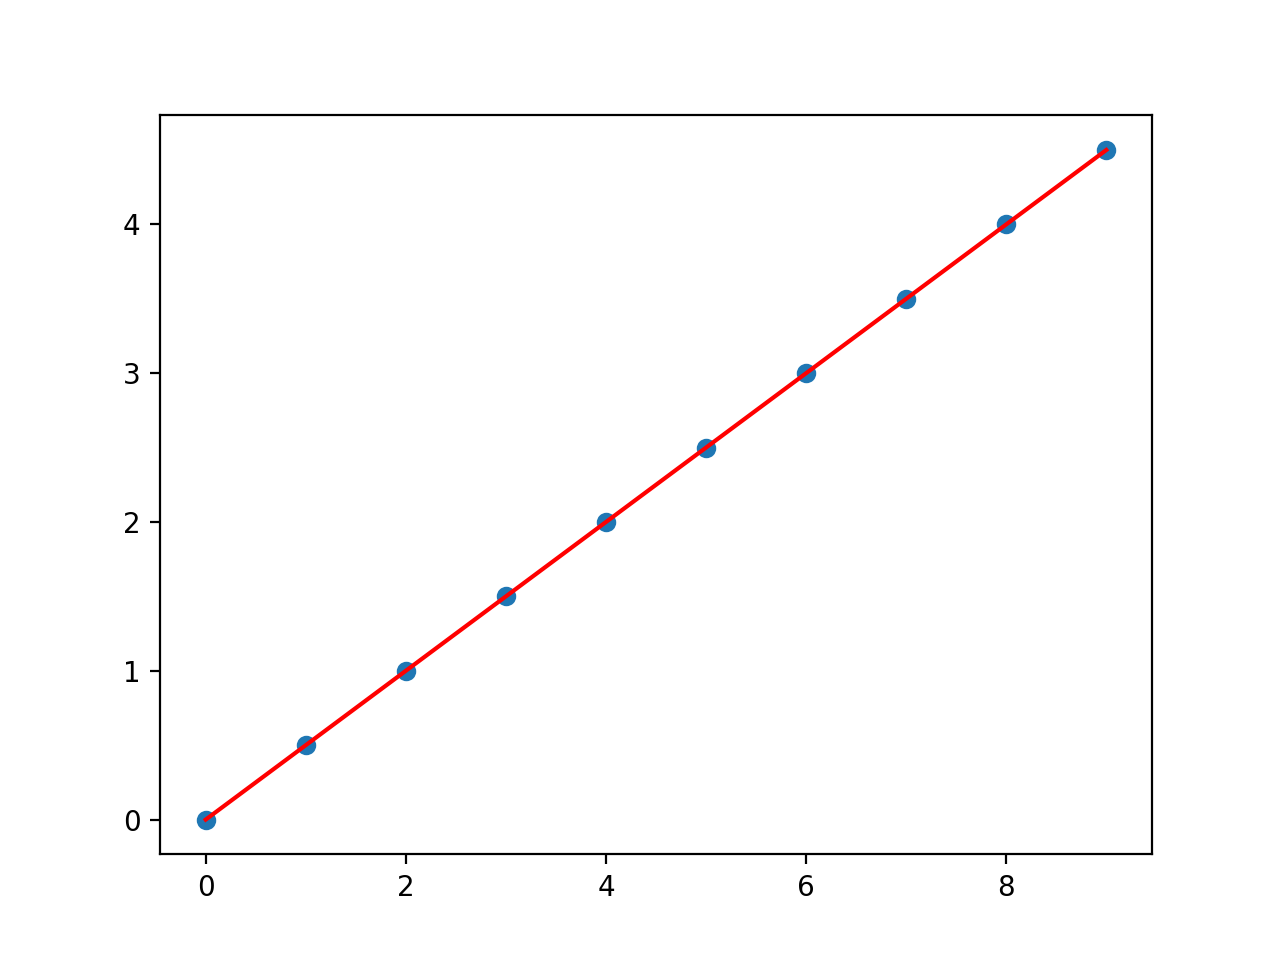
\includegraphics[height=0.5\textheight]{closedForm1D}
	\nextproblem
	2D-noisy-lin.txt
	\\ Closed form theta: [2.93987438] [2.04156149] [-0.43683838]
	\\ Closed form loss: 0.10759283475200873
	\\ Theoretical theta: [2.93987438] [2.04156149] [-0.43683838]
	\\ Theoretical loss: 0.10759283475200876
	\\ 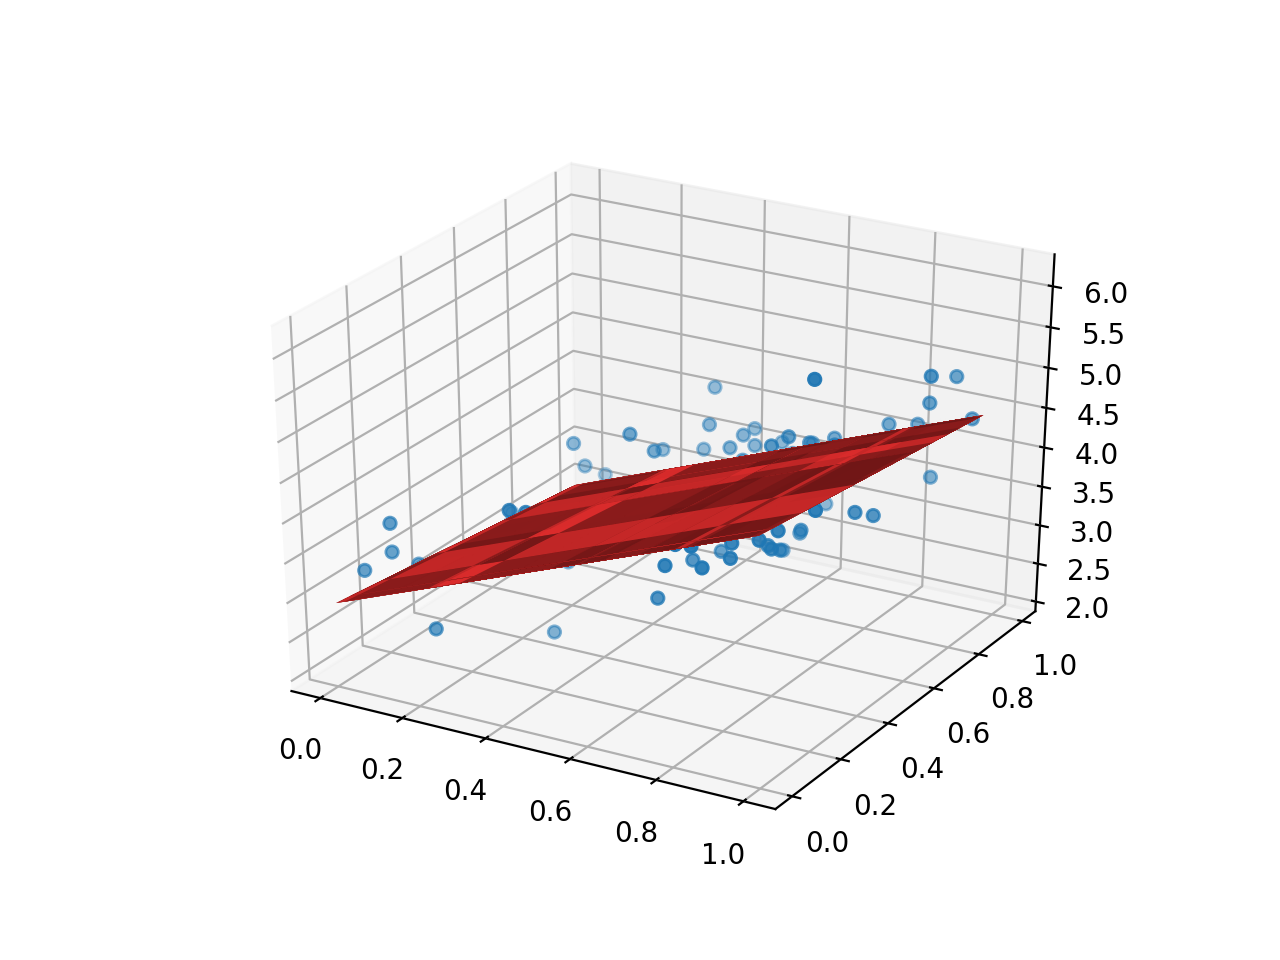
\includegraphics[height=0.5\textheight]{closedForm2D.png}
	\item When a feature of X is identical to another, it means that we will get a sigular matrix when performing $X^T X$ in closed form linear regression. A singular matrix does not have an inverse and thus we can not calculate theta. If there are duplicate features, that means there is are two identical columns in X. This makes $X^TX$ have n-1 pivot points which makes it not an invertible matrix. 
	\item When a training point of X is duplicated, it affects the values of the thetas that the closed form liinear regression predicts. Duplicating a training example means that during the loss calculation, there will be double the loss associate with this training point. Thus, the linear regression will change the thetas to minimize the loss at the duplicated training example. 
	\item For a duplicate feature, gradient descent will not run into the problem of trying to invert a non-invertible matrix but will have different results. The extra feature pushes the training examples closer together to form a line. For the 2D data, the points were pushed together, distincly forming a line shape. 
	\\ For a duplicate training point, gradient descent's loss function will also emphasize minimizing the doubled cost for the duplicate training example and thus will output different thetas than if X did not have the duplicate training example.
\end{enumerate}

\item 
\begin{enumerate}
	\item {Iteration: 1 , Loss: 3.5625 , Theta: [[0.] [0.]]
   \\ Iteration: 2 , Loss: 0.7573828125000001 , Theta: [[0.1125] [0.7125]]
   \\ Iteration: 3 , Loss: 0.16152348632812494 , Theta: [[0.0590625] [0.384375 ]]
   \\ Iteration: 4 , Loss: 0.03493766798400873 , Theta: [[0.082125  ] [0.53585156]]
	\\ Iteration: 5 , Loss: 0.008031704149217576 , Theta: [[0.06995215] [0.46628496]]
	\\ Iteration: 6 , Loss: 0.00229943603847955 , Theta: [[0.07404042] [0.49858966]]
	\\ Iteration: 7 , Loss: 0.0010651959009328556 , Theta: [[0.07065573] [0.4839403 ]]
	\\ Iteration: 8 , Loss: 0.0007868575553308054 , Theta: [[0.07073638] [0.49092783]]
	\\ Iteration: 9 , Loss: 0.0007120176497808081 , Theta: [[0.0692408 ] [0.48793999]]
	\\ Iteration: 10 , Loss: 0.0006808439364351451 , Theta: [[0.06849226] [0.48954633]]}
	\item \textbf{Running with default params for 1D-no-noise-lin.txt}
	\\ Gradient Descent Loss: 6.017302596643075e-10 , 
	\\ Gradient Descent Theta: [[6.44700512e-05] [4.99989719e-01]]
	\\ Closed form theta: [0.] [0.5]
	\\ Closed form loss: 0.0
	\\ \\ Running gradient descent with 500 iterations brought us very close to the same model parameters as closed form linear regression with an insignificant error of e-05 and e-01. The loss and thetas were essentially equal. The miniscule difference is caused because as gradient descent converges, it slows. 
	\\ \textbf{Running with default params for 2D-noisy-lin.txt}
	\\ Gradient Descent Loss: 0.11078751710215208 , 
	\\ Gradient Descent Theta: [[ 2.75594278] [ 2.09675389] [-0.16343704]]
	\\ Closed form theta: [2.93987438] [2.04156149] [-0.43683838]
	\\ Closed form loss: 0.10759283475200873
	\\ \\ Running gradient descent for the 2D data returned thetas and losses very close to what we got from closed form linear regression.
	\item \textbf{Learning rate, num iterations for 1D-no-noise-line.txt}
	\\ \textbf{alpha=[0.01, 0.05], num\_iters=[5, $\infty]$:}
	\\ This set of alphas and iterations give thetas and losses pretty much the same as the theoretical thetas and losses from closed form linear regression.
	\\ \textbf{alpha=[0.06, $\infty$], num\_iters=[1, $\infty]$:}
	\\ This set of alphas and iterations give thetas and losses noticeably different from the theoretical thetas and losses from closed form linear regression.
	\\ \textbf{Analysis:} It is noticeable that there is a pretty strict bound on learning rate if we are to obtain the optimal values. Learning rate is bound to the smaller numbers because relatively large learning rates can cause gradient descent to diverge. This is when the learning rate is so big that one iteration of gradient descent overshoots it's target. If the learning rate is realtively small, then each iteration of gradient descent will converge towards the global optimum. This is why the iteration number is less bound once you have an idea/non-idea alpha. There is also the set (not mentioned) which alpha is too small and converges very slowly. Given enough iterations, this will evertually converge to the global minimum. 
	\\ \textbf{alpha=[0.1, 1.2], num\_iters=[600, $\infty]$:}
	\\ This set of alphas and iterations give thetas and losses pretty much the same as the theoretical thetas and losses from closed form linear regression.
	\\ \textbf{alpha=[1.3, $\infty$], num\_iters=[1, $\infty]$:}
	\\ This set of alphas and iterations give thetas and losses noticeably different from the theoretical thetas and losses from closed form linear regression.
	\\ \textbf{Analysis:} The results and speculations for those results are similar to those of 1D, except that the learning rate bounds have a bigger range and value. It is evident that the 2D data set needed a lot more  iterations to converge to the global optimum. This could be caused by the fact that the slope between training examples is smaller. This can cause gradient descent with a smaller learning rate to converge very slowly. 
	\\ \textbf{Analysis on Divergence:} The reason why divergene happens is for each iteration of gradient descent, the thetas are moving further and further away from the optimum. Looking back on the step history, we can see that the large learning rate is causing theta values to alternate between positive and negative, increasing the loss with each iteration. 
\end{enumerate}
\nextproblem
\item
\begin{enumerate}
	\item \textbf{1D-exp-samp.txt}
	\\ K = 10
	\\ 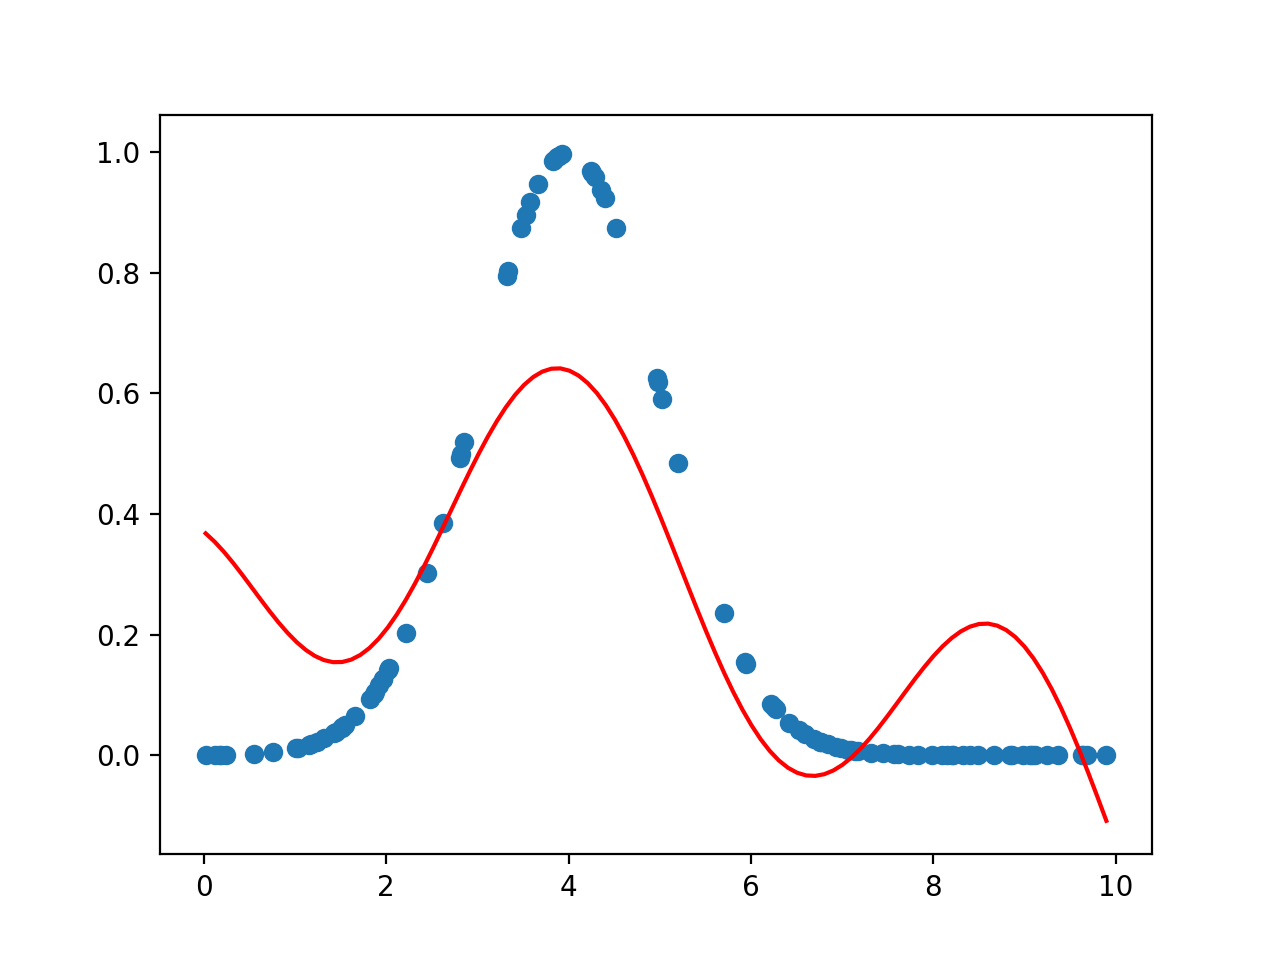
\includegraphics[height=0.3\textheight]{1Dexpsamp10}
	\\ K = 100
	\\ 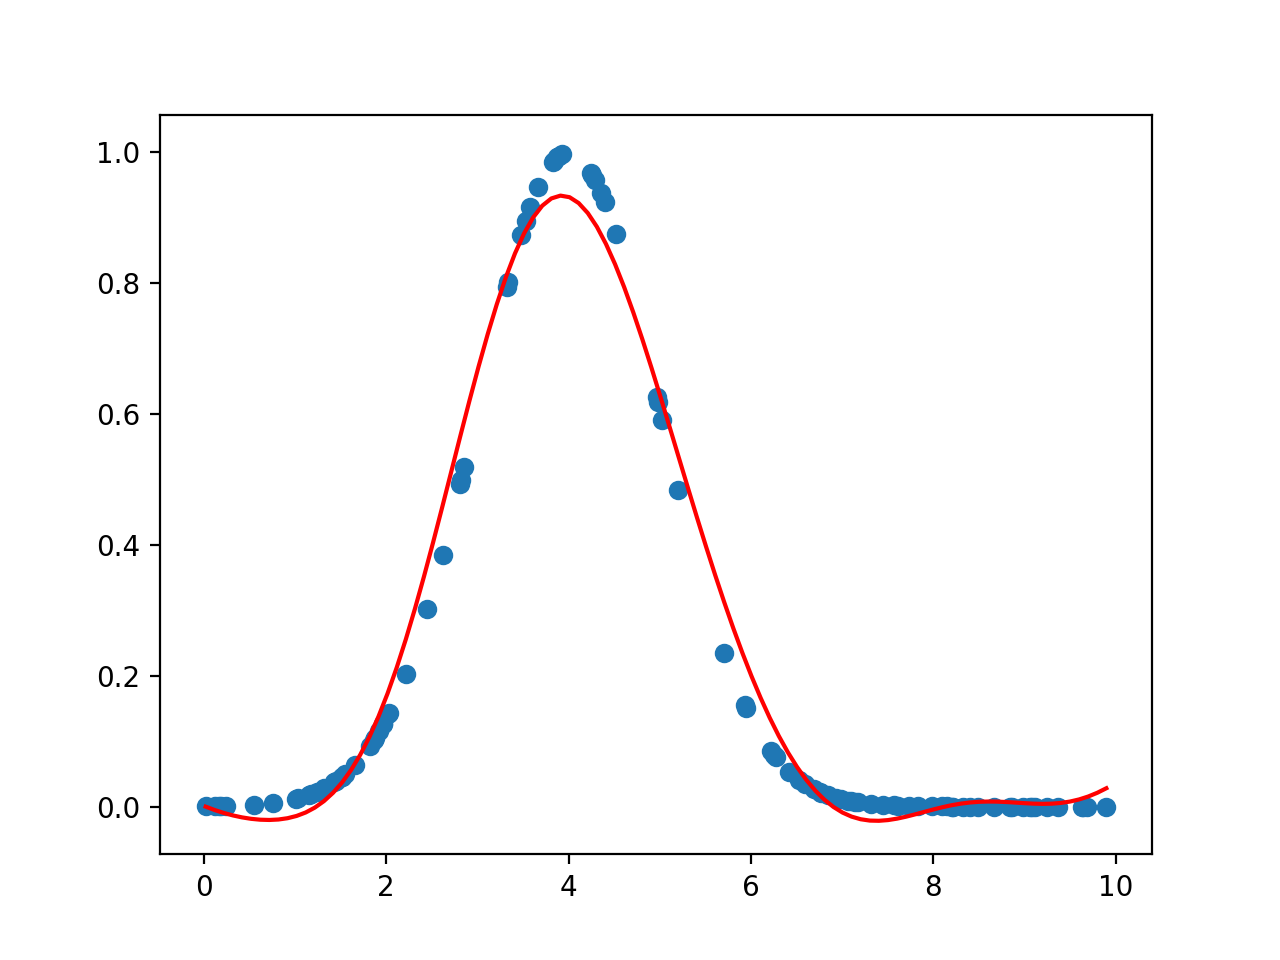
\includegraphics[height=0.3\textheight]{1Dexpsamp100}
	\\ K = 1000
	\\ 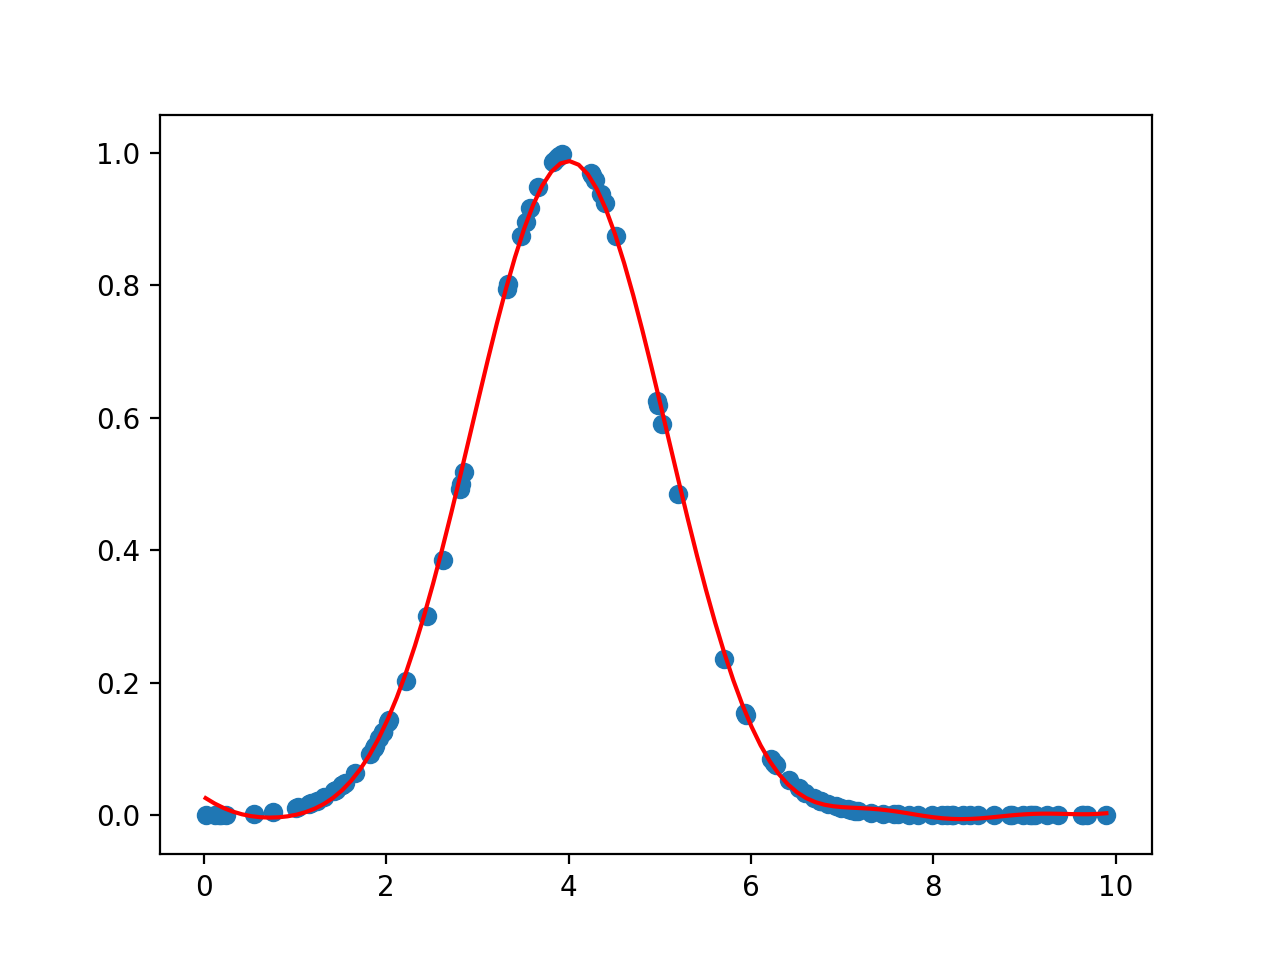
\includegraphics[height=0.3\textheight]{1Dexpsamp1000}
	\nextproblem
	\textbf{1D-exp-uni.txt}
	\\ K = 10
	\\ 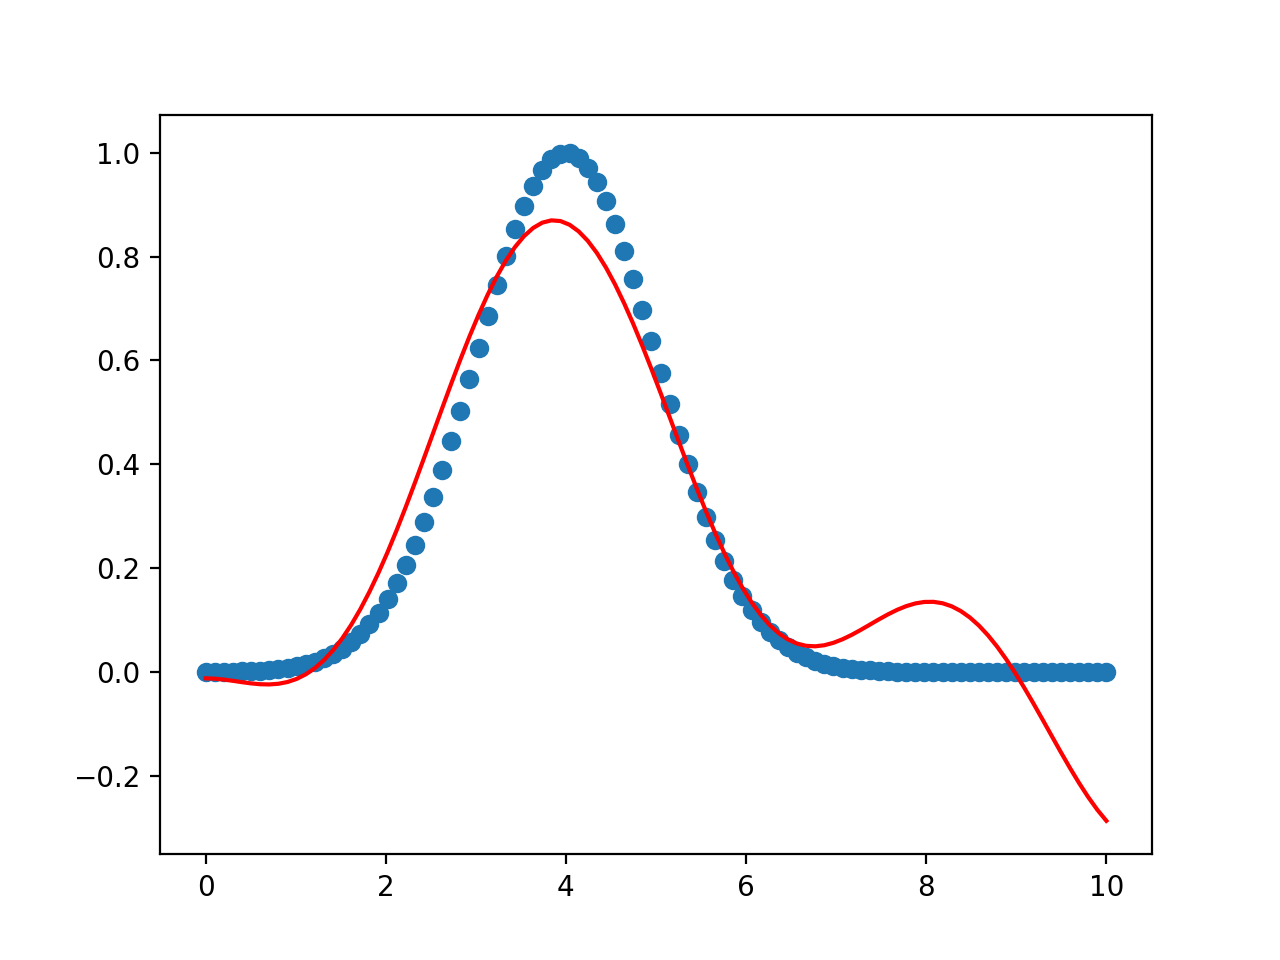
\includegraphics[height=0.3\textheight]{1Dexpuni10}
	\\ K = 50
	\\ 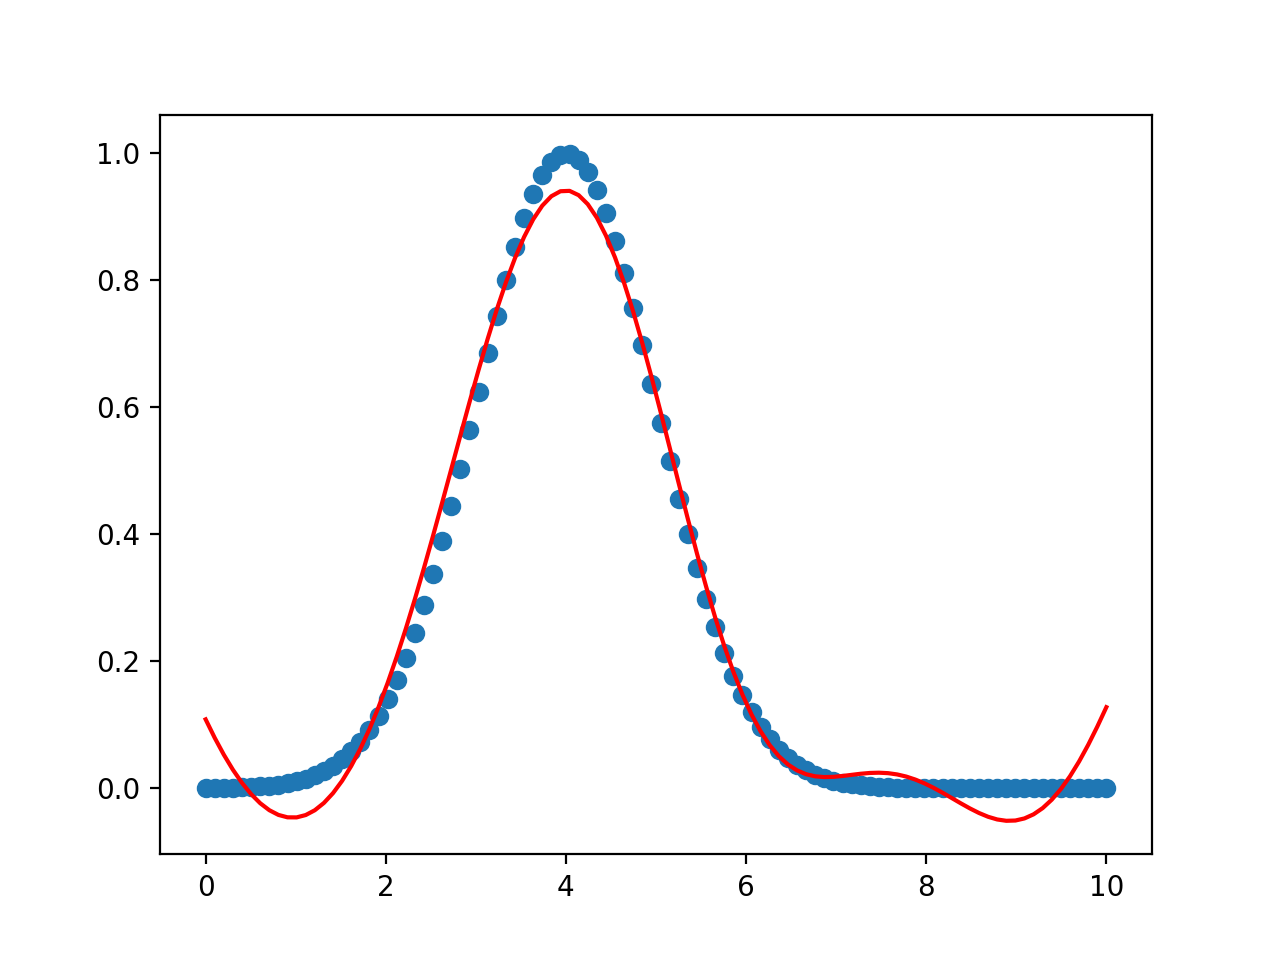
\includegraphics[height=0.3\textheight]{1Dexpuni50}
	\\ K = 800
	\\ 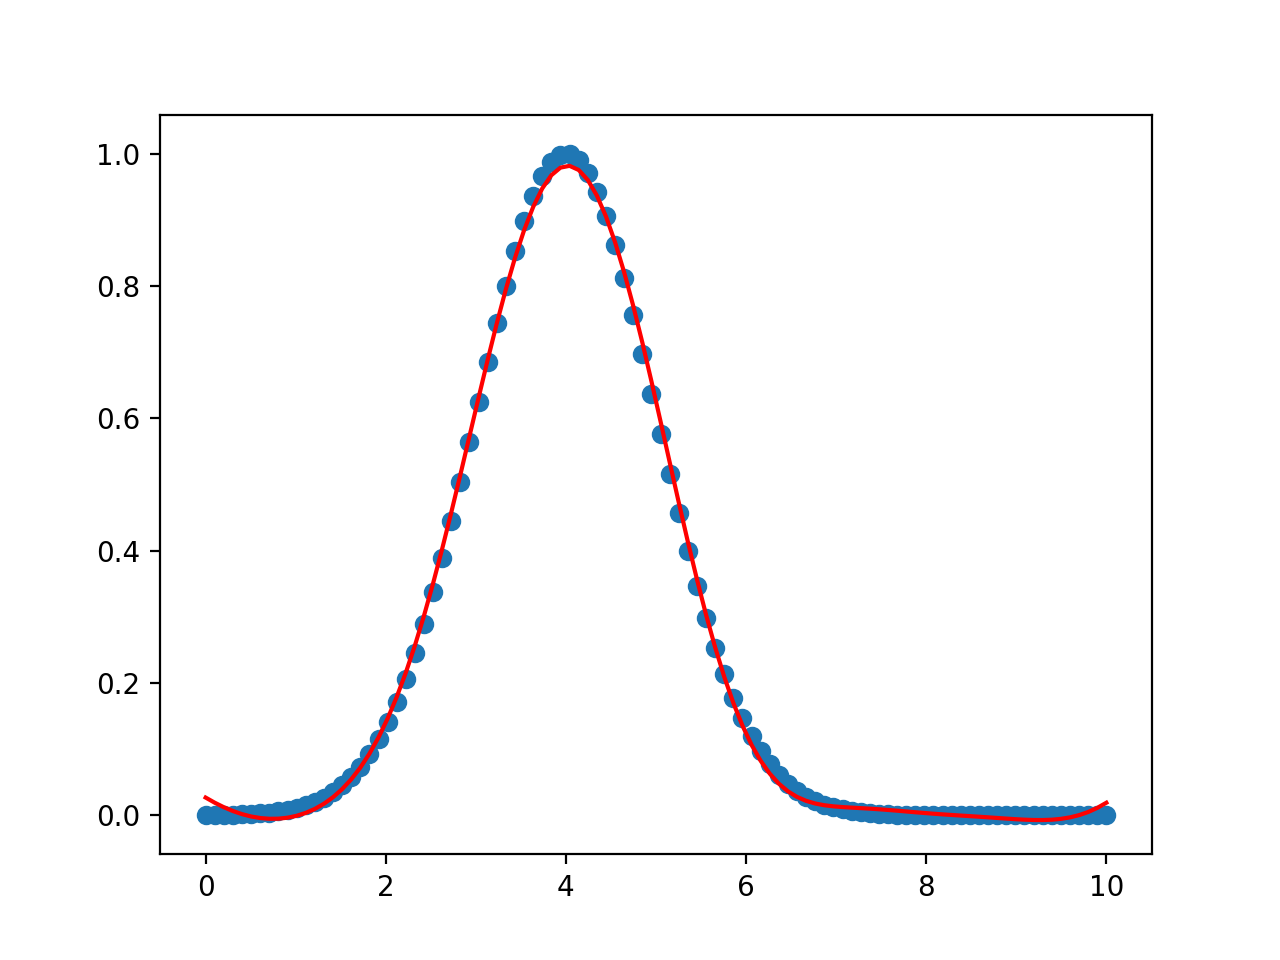
\includegraphics[height=0.3\textheight]{1Dexpuni800}
	\nextproblem
	\textbf{1D-quad-uni.txt}
	\\ K = 10
	\\ 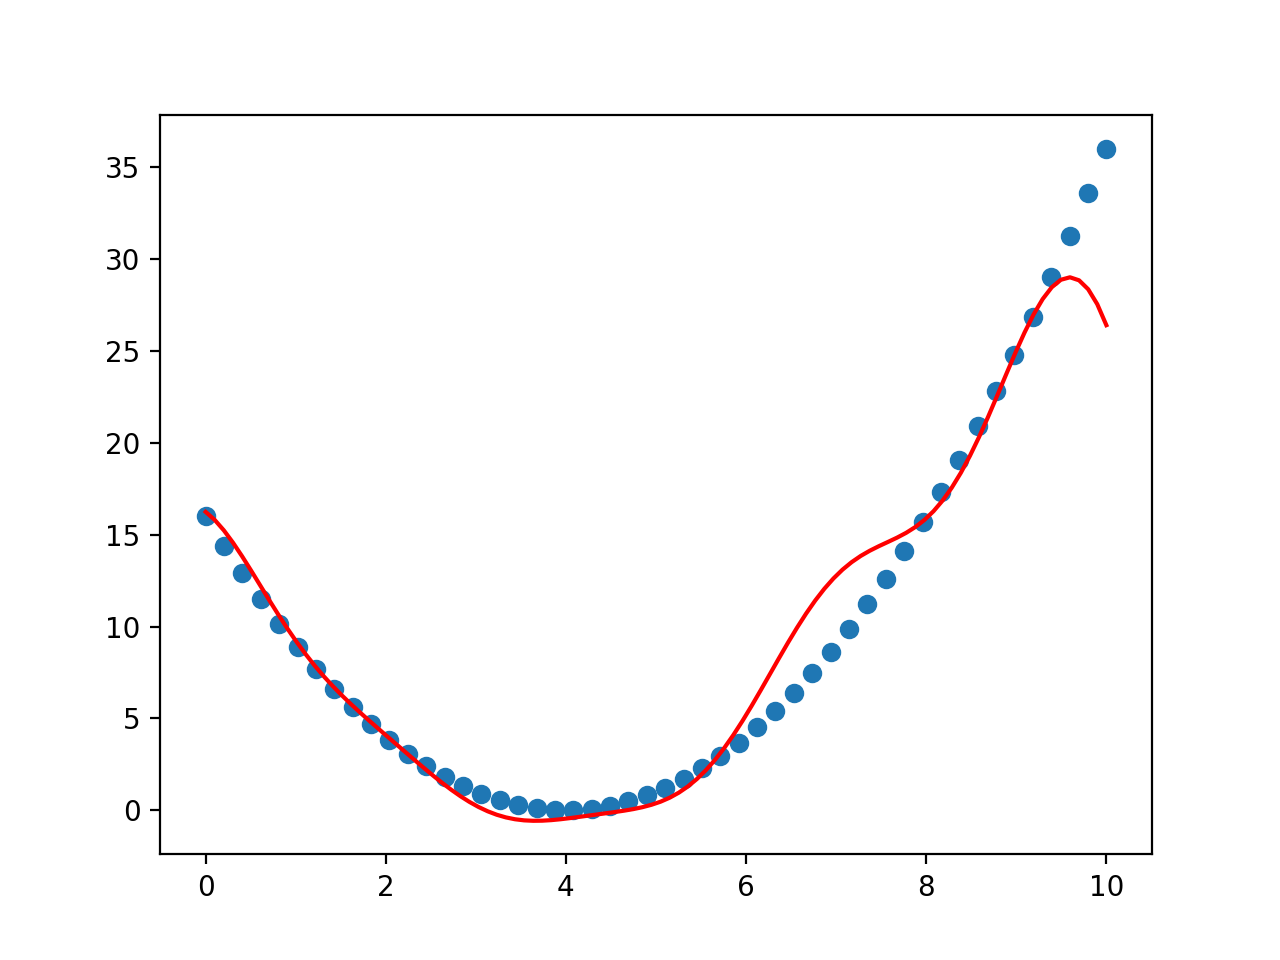
\includegraphics[height=0.3\textheight]{1Dquaduni10}
	\\ K = 50
	\\ 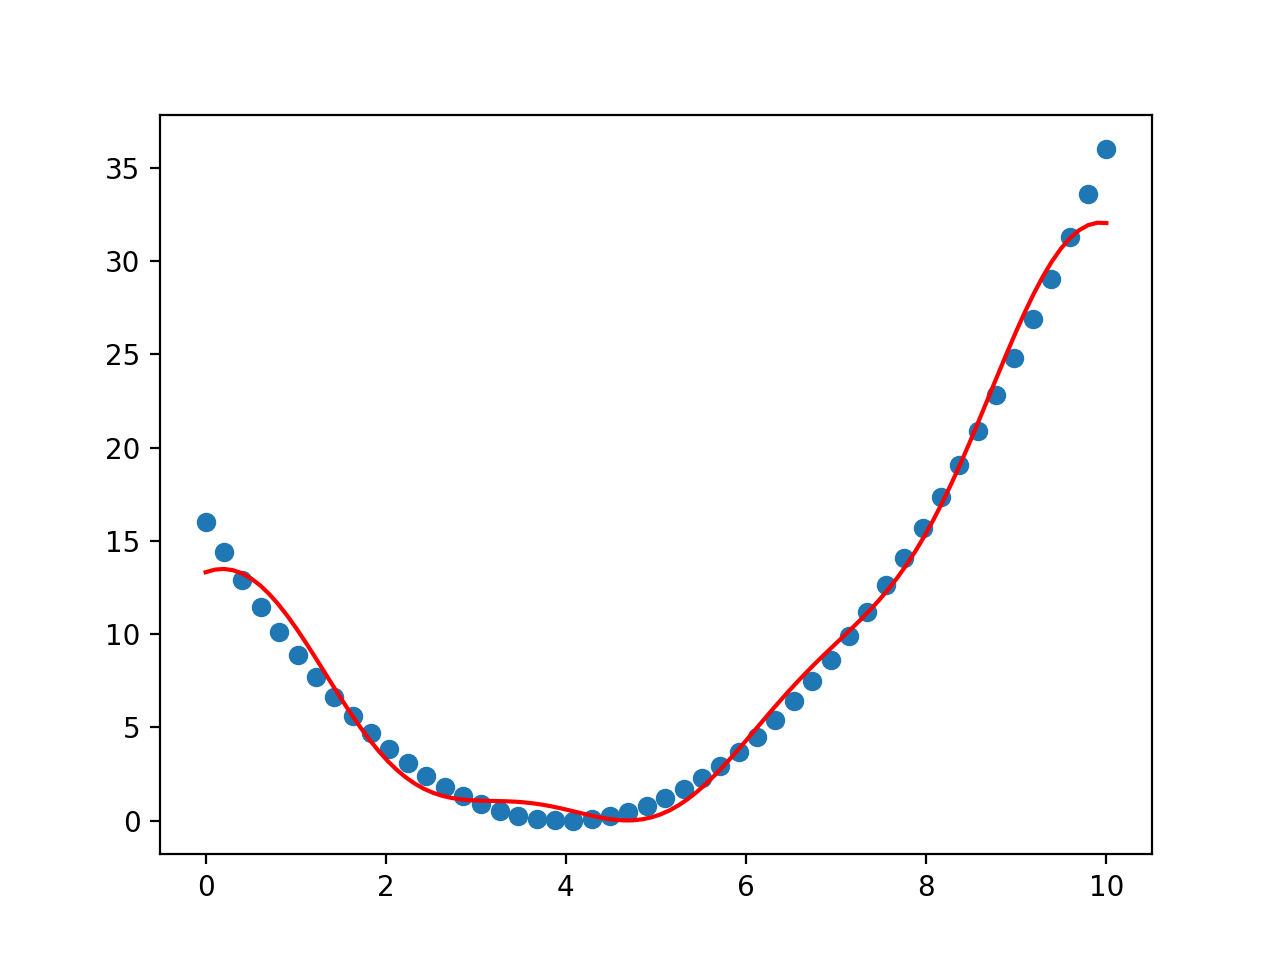
\includegraphics[height=0.3\textheight]{1Dquaduni50}
	\\ K = 800
	\\ 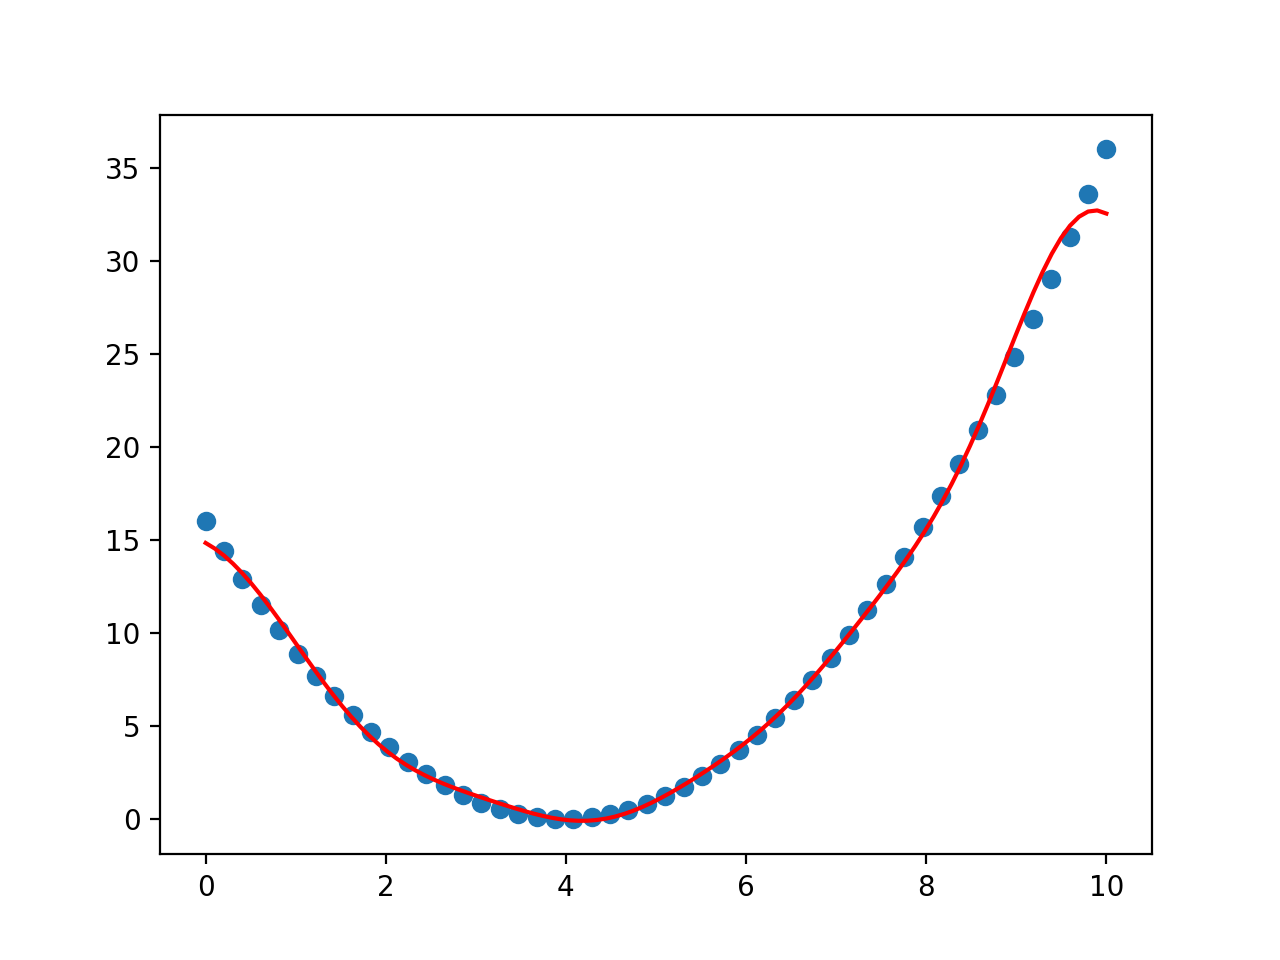
\includegraphics[height=0.3\textheight]{1Dquaduni800}
	\nextproblem
	\textbf{1D-exp-samp.txt}
	\\ K = 10
	\\ 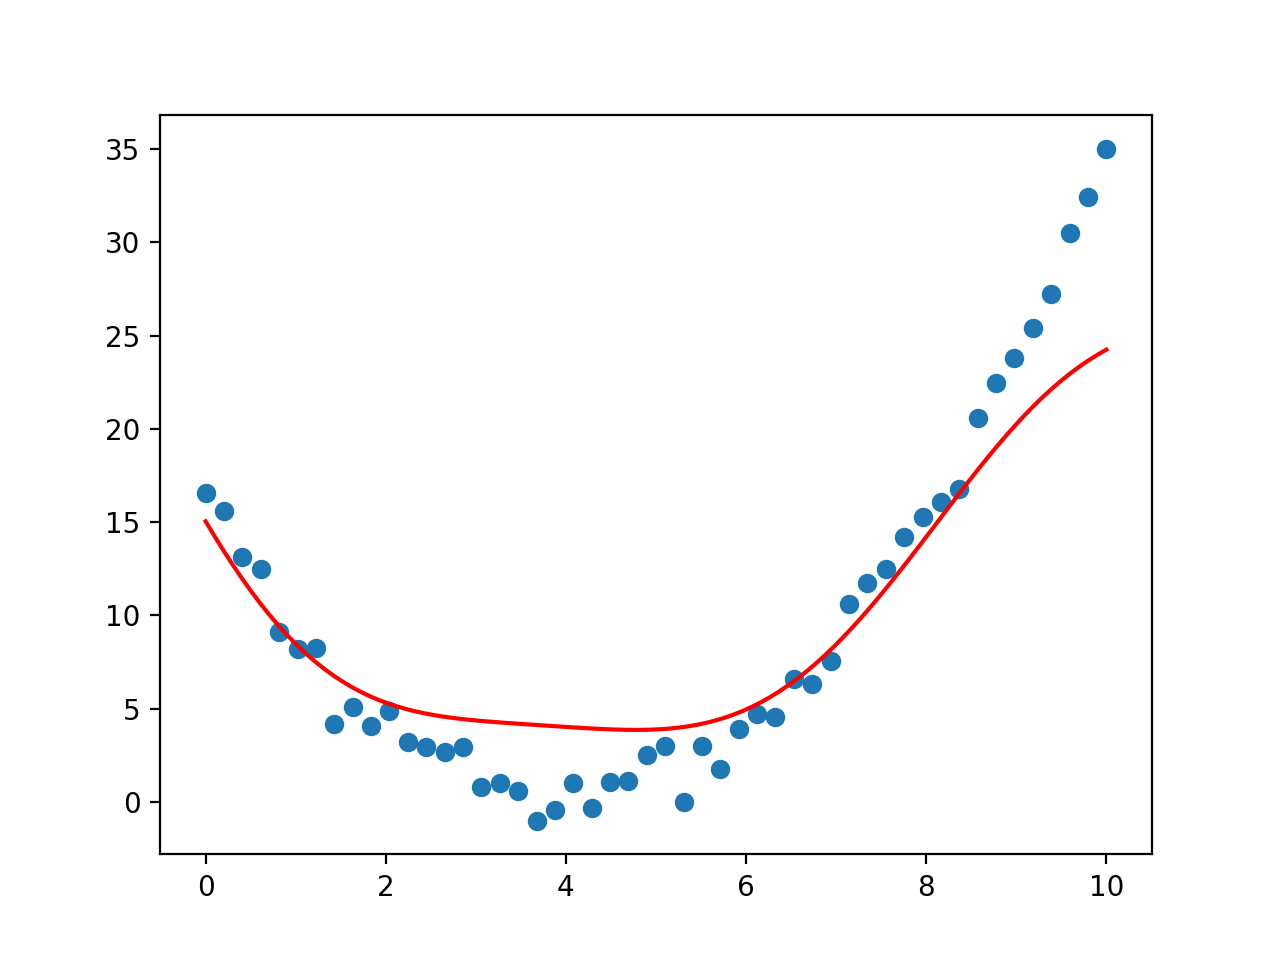
\includegraphics[height=0.3\textheight]{1Dquaduninoise10}
	\\ K = 100
	\\ 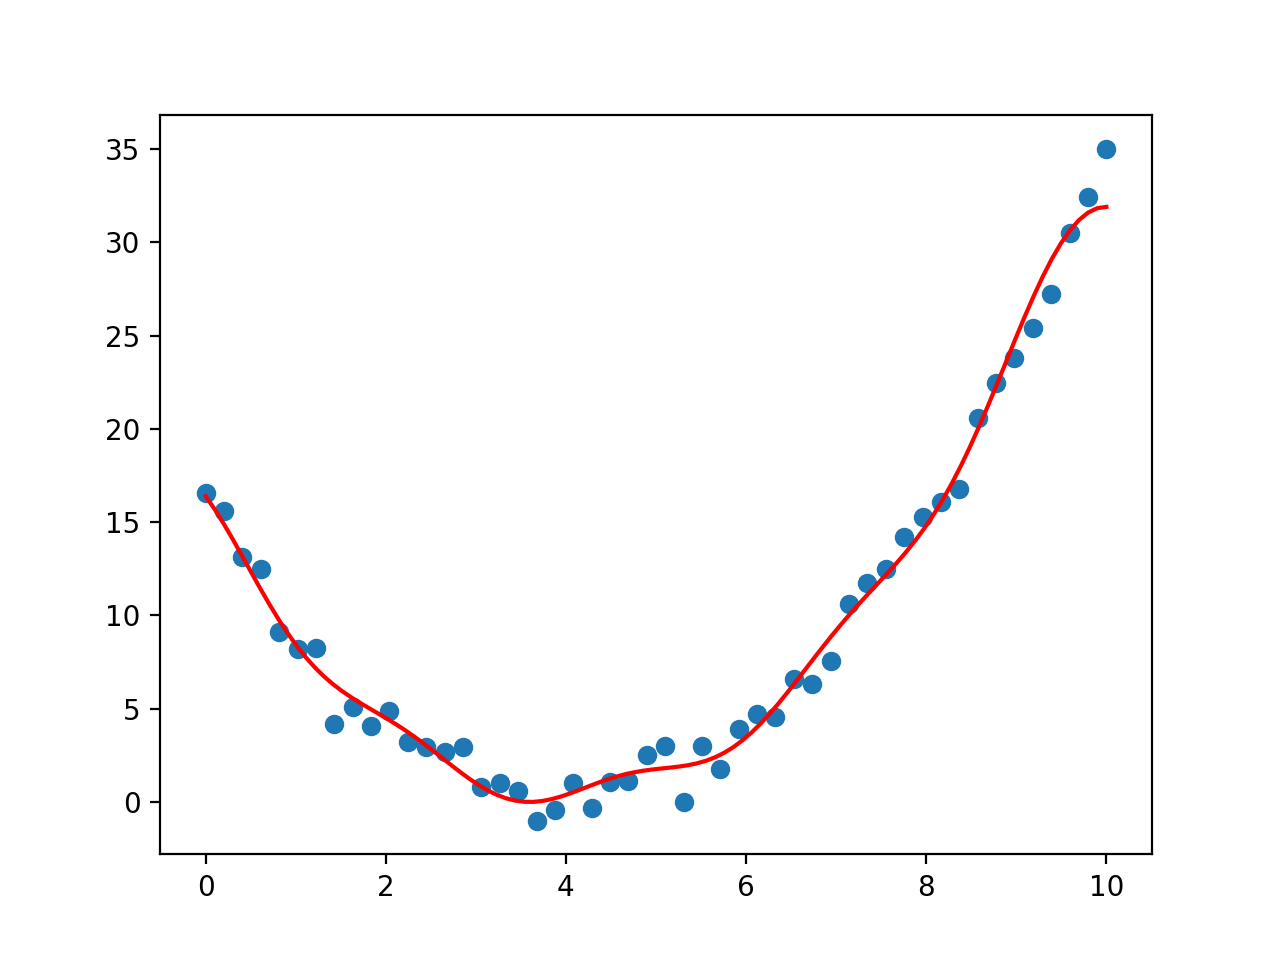
\includegraphics[height=0.3\textheight]{1Dquaduninoise100}
	\\ K = 1000
	\\ 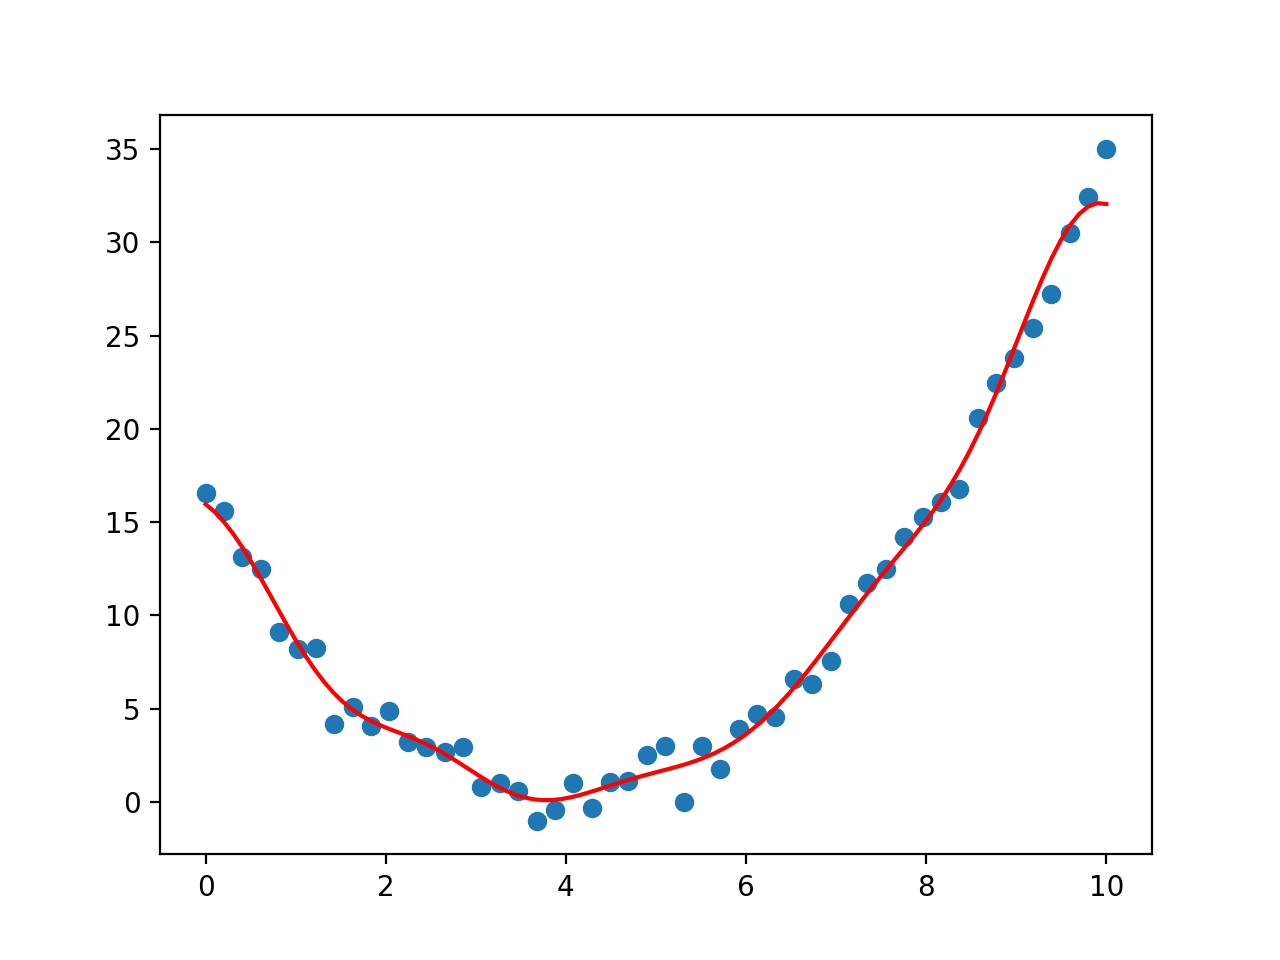
\includegraphics[height=0.3\textheight]{1Dquaduninoise1000}
	\nextproblem
	\item \textbf{Extra Credit}
	\\ I believe that if you predict a value far from the training data set with RFF, it might predict correctly depending on where the point is. The way how RFF works is that it randomly samples the kernel (in our case it's the cosine function) with varying offsets and frequencies. Then it takes these sampled bits of the function and uses gradient descent to obtain theta values that are essentially weights for the sampled functions. The thetas attempt to fit a function into the shape of the training dataset. Because of this process, at the bounds of the dataset, the prediction will fluxuate in a pattern reminiscent of the majority of the data set as it tries to predict the new outlying point. For example with the 1D dataset, if the point is within the y bounds of the dataset, the model might be able to predict somewhat the point but with still significant loss. If the point is within the bounds of x but far away from y, then the loss associated with this point will be huge. It still will pull the model towards it but it will still have a massive loss value.
\end{enumerate}

\end{enumerate}

\end{document}

